\chapter{Microservicios Spring Cloud}
\section{Aplicaciones con Java EE.}
La aplicaci\'on necesita una versi\'on est\'andar de Java SE para ejecutarse.Con Java EE siguiendo
el est\'andar se evita el vendor looking ,es decir aferarse a una sola tecnolog\'\i{}a o proveedor.\\
Servidor de aplicaciones : Contenedor que cumple con las especificaciones de Java EE.\\
Ejemplo : Jboss,Wildfly,Glassfish .\\
Servidor web :Ofrece APIS de servelets,jsps.Se puede A\~nadir otras librer\'\i{}as Java EE.Son servidores ligeros.\\
Ejemplo : Tomcat,Jetty.
\section{Spring.}
Es un framework de desarrollo de aplicaciones empresariales.Sus partes est\'an basadas sobre Java EE .\\
Permite desarrollar aplicaciones Rest,web sockets,an\'alisis de bigdata.Proceso de tareas por lote (Bath).\\
Soporte a base de datos SQL y NoSQL.\\
Soporte de arquitecturas reactivas con reactor.
\section{Spring Boot.}
Facilita el desarrollo de aplicaciones con spring.El servidor tomcat esta embebido.\\
Simplifica la configuraci\'on, ya no se usa ficheros xml.
\section{Maven.}
Sistema de gesti\'on de dependencias y de construcci\'on de proyectos.\\
Compatible con todos los entornos de desarrollo y sistemas de integraci\'on continua.
\section{Spring Tool Suite STS.}
Proporciona facilidades para trabajar con aplicaciones spring.\\
Cuando se hace cambios en el fichero pom.xml a veces ocurre que los cambios no ocurren en eclipse de manera autom\'atica.
Para solucionar esto,bot\'on derecho proyecto,maven,update Project.
\section{Spring MVC.}
Sigue la arquitectura MVC  y sirve para la construcci\'on de aplicaciones webs.
\section{Microservicios.}
Son un conjunto de componentes peque\~nos y aut\'onomos que colaboran entre si.\\
Carateristicas:
\begin{itemize}
	\item Funci\'on \'unica.
	\item Son independientes.
	\item Registro y autodescubrimiento del servicio.
	\item Escalado  y agilidad.
	\item Confibialidad y tolerancia a fallos.(Timeout,servicio alternativo,evitar errores en cascada).
	\item Balanceo de carga.
	\item Autonomos son independientes,especializados,escalables,balance de carga,agilidad y equipos  mas peque\~nos.ciclo de desarrollo mas corto, c\'odigo reutilizable.Independencia tecnologtica, es decir cada servicio puede usar su propia librer\'\i{}a
	\item .
\end{itemize}

\section{Spring Cloud.}
Trabaja con programacion reactiva asíncrono,no bloqueantes.
\section{Servidor Eureka.}
Es para registrar los microservicios,cada servicio tiene un identificador \'unico.Cada servicio debe 
ser un cliente de Eureka.\\
Balanceo de carga Ribbon,spring cloud load balance.
\section{API Gateway.}
Se encarga del enrutamiento dinamico.
\section{Zeul  Netflix.}
Trabaja con API serlets un hilo por request.Bloqueantes un proceso por una tarea.
\begin{figure}[H] 
	\centering
	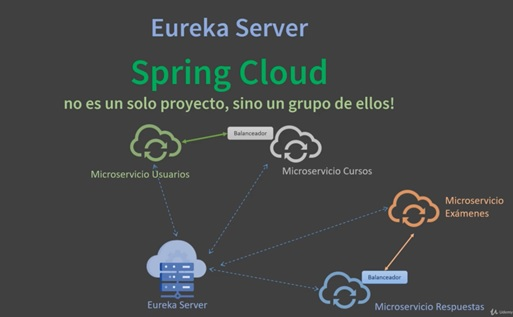
\includegraphics[scale=0.7]{images/c2_1.jpg}
	\caption{Eureka server.}
\end{figure}
\section{API Gateway.}
Zuul Netflix y Spring Cloud Gateway.\\
Puerta de enlace,acceso centralizado.\\
Enrutamiento dinamico de los microservicios.\\
Balanceo de carga.\\
Maneja filtros propios.\\
Permite extender funcionalidades.\\
BBD Compartida.\\
Ventajas:
\begin{itemize}
	\item Transacciones ACID.
	\item Mejor integridad de datos.
	\item Una sola base de datos es mas f\'acil de operar.
\end{itemize}
Desventajas:
Ventajas:
\begin{itemize}
	\item Mayor acoplamiento de los servicios.
	\item Dificultad  el escalamiento de instancias.
	\item Las bds a veces se deben replicar y fragmentar para escalar..
\end{itemize}
\begin{figure}[H] 
	\centering
	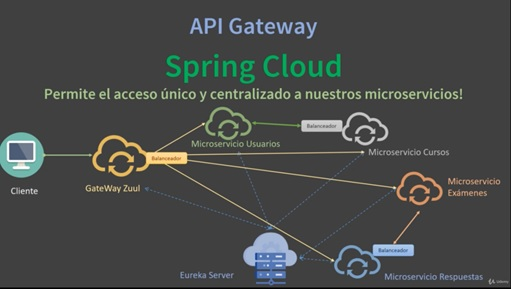
\includegraphics[scale=0.7]{images/c2_2.jpg}
	\caption{API Gateway.}
\end{figure}
\section{.}
\section{.}








